%package list
\documentclass{article}
\usepackage[top=3cm, bottom=3cm, outer=3cm, inner=3cm]{geometry}
\usepackage{multicol}
\usepackage{listings}
\usepackage[utf8]{inputenc}
\usepackage{graphicx}
\usepackage{url}
%\usepackage{cite}
\usepackage{hyperref}
\usepackage{array}
%\usepackage{multicol}
\newcolumntype{x}[1]{>{\centering\arraybackslash\hspace{0pt}}p{#1}}
\usepackage{natbib} 
\usepackage{pdfpages}
\usepackage{multirow}   
\usepackage[normalem]{ulem}
\useunder{\uline}{\ul}{}
\usepackage{svg}
\usepackage{xcolor}
\usepackage{listings}
\lstdefinestyle{ascii-tree}{
    literate={├}{|}1 {─}{--}1 {└}{+}1 
  }
\lstset{basicstyle=\ttfamily,
  showstringspaces=false,
  commentstyle=\color{red},
  keywordstyle=\color{blue}
}
%\usepackage{booktabs}
\usepackage{caption}
\usepackage{subcaption}
\usepackage{float}
\usepackage{array}

\newcolumntype{M}[1]{>{\centering\arraybackslash}m{#1}}
\newcolumntype{N}{@{}m{0pt}@{}}


%%%%%%%%%%%%%%%%%%%%%%%%%%%%%%%%%%%%%%%%%%%%%%%%%%%%%%%%%%%%%%%%%%%%%%%%%%%%
%%%%%%%%%%%%%%%%%%%%%%%%%%%%%%%%%%%%%%%%%%%%%%%%%%%%%%%%%%%%%%%%%%%%%%%%%%%%
\newcommand{\itemEmail}{ shanccom@unsa.edu.pe
}
\newcommand{\itemStudent}{ Sergio Hancco Mullisaca }
\newcommand{\itemCourse}{Programacion Web 2}
\newcommand{\itemCourseCode}{}
\newcommand{\itemSemester}{II}
\newcommand{\itemUniversity}{Universidad Nacional de San Agustín de Arequipa}
\newcommand{\itemFaculty}{Facultad de Ingeniería de Producción y Servicios}
\newcommand{\itemDepartment}{Departamento Académico de Ingeniería de Sistemas e Informática}
\newcommand{\itemSchool}{Escuela Profesional de Ingeniería de Sistemas}
\newcommand{\itemAcademic}{2024 - A}
\newcommand{\itemInput}{Del 26 Mayo 2024}
\newcommand{\itemOutput}{Al 29 Mayo 2024}
\newcommand{\itemPracticeNumber}{6}
\newcommand{\itemTheme}{DJANGO}
%%%%%%%%%%%%%%%%%%%%%%%%%%%%%%%%%%%%%%%%%%%%%%%%%%%%%%%%%%%%%%%%%%%%%%%%%%%%
%%%%%%%%%%%%%%%%%%%%%%%%%%%%%%%%%%%%%%%%%%%%%%%%%%%%%%%%%%%%%%%%%%%%%%%%%%%%

\usepackage[english,spanish]{babel}
\usepackage[utf8]{inputenc}
\AtBeginDocument{\selectlanguage{spanish}}
\renewcommand{\figurename}{Figura}
\renewcommand{\refname}{Referencias}
\renewcommand{\tablename}{Tabla} %esto no funciona cuando se usa babel
\AtBeginDocument{%
	\renewcommand\tablename{Tabla}
}

\usepackage{fancyhdr}
\pagestyle{fancy}
\fancyhf{}
\setlength{\headheight}{30pt}
\renewcommand{\headrulewidth}{1pt}
\renewcommand{\footrulewidth}{1pt}
\fancyhead[L]{\raisebox{-0.2\height}{\includegraphics[width=3cm]{logo_episunsa.png}}}
\begin{figure}
    \centering
    \label{fig:enter-label}
\end{figure}
\fancyhead[C]{\fontsize{7}{7}\selectfont	\itemUniversity \\ \itemFaculty \\ \itemDepartment \\ \itemSchool \\ \textbf{\itemCourse}}
\fancyhead[R]{\raisebox{-0.2\height}{\includegraphics[width=1.2cm]{}}}
\fancyfoot[C]{\itemCourse}
\fancyfoot[R]{Página \thepage}

% para el codigo fuente
\usepackage{listings}
\usepackage{color, colortbl}
\definecolor{dkgreen}{rgb}{0,0.6,0}
\definecolor{gray}{rgb}{0.5,0.5,0.5}
\definecolor{mauve}{rgb}{0.58,0,0.82}
\definecolor{codebackground}{rgb}{0.95, 0.95, 0.92}
\definecolor{tablebackground}{rgb}{0.8, 0, 0}

\lstset{frame=tb,
	language=bash,
	aboveskip=3mm,
	belowskip=3mm,
	showstringspaces=false,
	columns=flexible,
	basicstyle={\small\ttfamily},
	numbers=none,
	numberstyle=\tiny\color{gray},
	keywordstyle=\color{blue},
	commentstyle=\color{dkgreen},
	stringstyle=\color{mauve},
	breaklines=true,
	breakatwhitespace=true,
	tabsize=3,
	backgroundcolor= \color{codebackground},
}

\begin{document}
	
	\vspace*{10px}
	
	\begin{center}	
		\fontsize{17}{17} \textbf{ Informe de Laboratorio \itemPracticeNumber}
	\end{center}
	\centerline{\textbf{\Large Tema: \itemTheme}}
	%\vspace*{0.5cm}	

	\begin{flushright}
		\begin{tabular}{|M{2.5cm}|N|}
			\hline 
			\rowcolor{tablebackground}
			\color{white} \textbf{Nota}  \\
			\hline 
			     \\[30pt]
			\hline 			
		\end{tabular}
	\end{flushright}	

	\begin{table}[H]
		\begin{tabular}{|x{4.7cm}|x{4.8cm}|x{4.8cm}|}
			\hline 
			\rowcolor{tablebackground}
			\color{white} \textbf{Estudiante} & \color{white}\textbf{Escuela}  & \color{white}\textbf{Asignatura}   \\
			\hline 
			{\itemStudent \par \itemEmail} & \itemSchool & {\itemCourse \par Semestre: \itemSemester \par Código: \itemCourseCode}     \\
			\hline 			
		\end{tabular}
	\end{table}		
	
	\begin{table}[H]
		\begin{tabular}{|x{4.7cm}|x{4.8cm}|x{4.8cm}|}
			\hline 
			\rowcolor{tablebackground}
			\color{white}\textbf{Laboratorio} & \color{white}\textbf{Tema}  & \color{white}\textbf{Duración}   \\
			\hline 
			\itemPracticeNumber  & \itemTheme & 04 horas   \\
			\hline 
		\end{tabular}
	\end{table}
	
	\begin{table}[H]
		\begin{tabular}{|x{4.7cm}|x{4.8cm}|x{4.8cm}|}
			\hline 
			\rowcolor{tablebackground}
			\color{white}\textbf{Semestre académico} & \color{white}\textbf{Fecha de inicio}  & \color{white}\textbf{Fecha de entrega}   \\
			\hline 
			\itemAcademic & \itemInput &  \itemOutput  \\
			\hline 
		\end{tabular}
	\end{table}
	
	\section{Tarea}
	\begin{itemize}		
		\item Informe de laboratorio
            \item Video en Flip
		\item Ejercicios Propuestos
        
	\end{itemize}
		
	\section{Equipos, materiales y temas utilizados}
	\begin{itemize}
		\item VS
		\item Git 2.39.2.
		\item Cuenta en GitHub con el correo institucional.
	\end{itemize}
    \clearpage
    
	\section{URL de Repositorio Github}
	\begin{itemize}
        \item URL del video en yt.
		\item \url{https://youtu.be/1L9XbhlCb8c}
        \item URL del video en flip.
		\item \url{https://flip.com/s/e5hcCChND88N}
        \item URL del GITHUB.
            \item \url{https://github.com/shanccom/Programacion_Web_2.git}
	\end{itemize}
	
	\section{Actividades}
	\subsection{EJERCICIO PROPUESTO}
        \item CREACION ENTORNO VIRTUAL CON GITIGNORE
        \newline \newline
        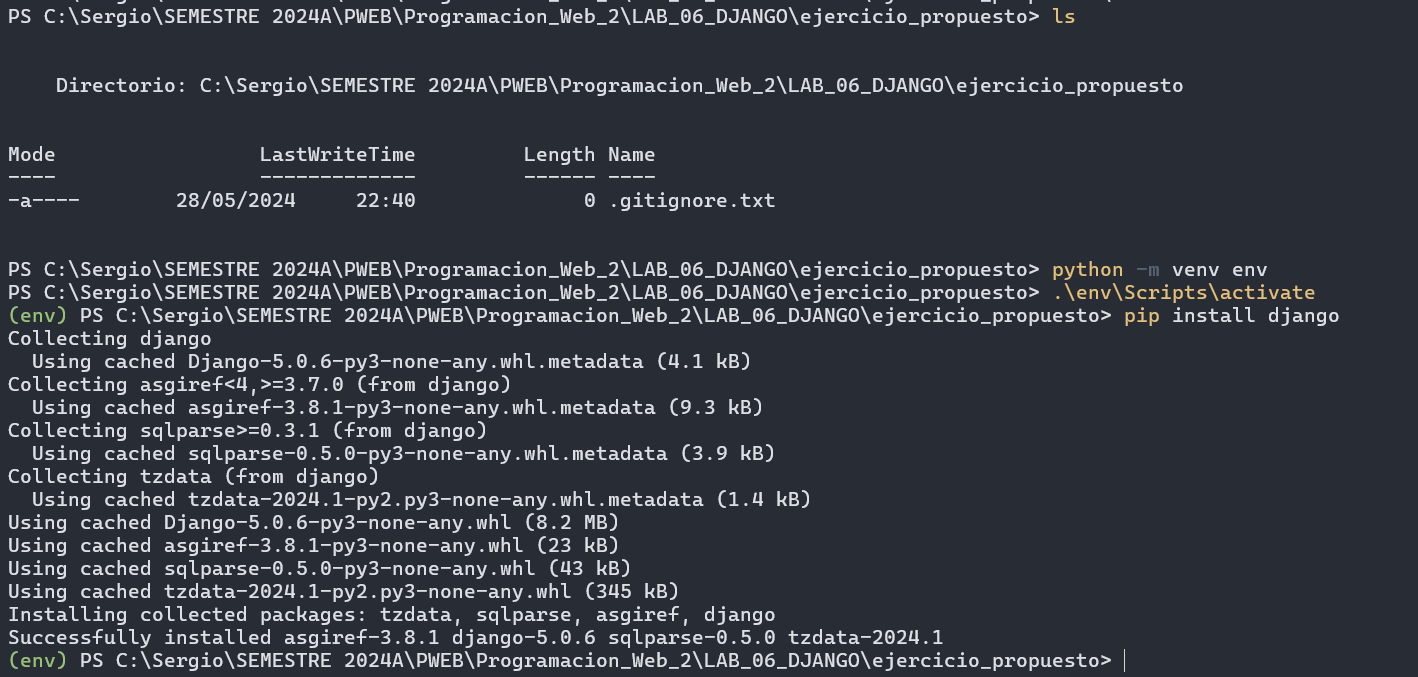
\includegraphics[width=0.8\textwidth,keepaspectratio]{Creacion entorno virtual.png}

        \item ARCHIVOS MODIFICADOS (app)
        
        \begin{lstlisting}[language=Python, caption=models.py]
from django.db import models

# Creacion de modelos propios

class Alumno(models.Model):
    nombre = models.CharField(max_length = 50)
    apellido = models.CharField(max_length = 50)
    cui = models.CharField(max_length = 8, unique = True)

    def __str__(self):
        return f"{self.nombre} {self.apellido}"

class Curso(models.Model):
    nombre = models.CharField(max_length=100)
    descripcion = models.TextField(blank=True)
    
    def __str__(self):
        return self.nombre

class NotasAlumno(models.Model):
    alumno = models.ForeignKey(Alumno, on_delete = models.CASCADE)
    curso = models.ForeignKey(Curso, on_delete = models.CASCADE)
    nota = models.DecimalField(max_digits = 5, decimal_places = 2)

    def __str__(self):
        return f"{self.alumno} - {self.curso}: {self.nota}"

        \end{lstlisting}  
        
        \begin{lstlisting}[language=Python, caption=admin.py]
from django.contrib import admin
from .models import Alumno, Curso, NotasAlumno

admin.site.register(Alumno)
admin.site.register(Curso)
admin.site.register(NotasAlumno)
        \end{lstlisting}
        
        \begin{lstlisting}[language=Python, caption=apps.py]
 from django.apps import AppConfig

class AdministracionConfig(AppConfig):
    default_auto_field = 'django.db.models.BigAutoField'
    name = 'administracion'
        \end{lstlisting}  
        \begin{lstlisting}[language=Python, caption=forms.py]
 from django import forms
from .models import Alumno, Curso, NotasAlumno

class AlumnoForm(forms.ModelForm):
    class Meta:
        model = Alumno
        fields = ['nombre', 'apellido', 'cui']

class CursoForm(forms.ModelForm):
    class Meta:
        model = Curso
        fields = ['nombre']

class NotasAlumnosPorCursoForm(forms.ModelForm):
    class Meta:
        model = NotasAlumno
        fields = ['alumno', 'curso', 'nota']
        \end{lstlisting}  

        \begin{lstlisting}[language=Python, caption=urls.py]
from django.urls import path
from .views import nuevo_alumno, nuevo_curso, nueva_nota, lista_alumnos, lista_cursos, lista_notas,eliminar_alumno, eliminar_curso, eliminar_nota

urlpatterns = [
    path('', nuevo_alumno, name='inicio'),
    path('nuevo_alumno/', nuevo_alumno, name='nuevo_alumno'),
    path('nuevo_curso/', nuevo_curso, name='nuevo_curso'),
    path('nueva_nota/', nueva_nota, name='nueva_nota'),
    path('lista_alumnos/', lista_alumnos, name='lista_alumnos'),
    path('lista_cursos/', lista_cursos, name='lista_cursos'),
    path('lista_notas/', lista_notas, name='lista_notas'),
    path('eliminar_alumno/<int:alumno_id>/', eliminar_alumno, name='eliminar_alumno'),
    path('eliminar_curso/<int:curso_id>/', eliminar_curso, name='eliminar_curso'),
    path('eliminar_nota/<int:nota_id>/', eliminar_nota, name='eliminar_nota'),

]   
        \end{lstlisting}  

        \begin{lstlisting}[language=Python, caption=views.py]
from django.shortcuts import render, redirect, get_object_or_404
from .forms import AlumnoForm, CursoForm, NotasAlumnosPorCursoForm
from .models import Alumno, Curso, NotasAlumno

def nuevo_alumno(request):
    if request.method == "POST":
        form = AlumnoForm(request.POST)
        if form.is_valid():
            form.save()
            return redirect('lista_alumnos')
    else:
        form = AlumnoForm()
    return render(request, 'administracion/nuevo_alumno.html', {'form': form})

def nuevo_curso(request):
    if request.method == "POST":
        form = CursoForm(request.POST)
        if form.is_valid():
            form.save()
            return redirect('lista_cursos')
    else:
        form = CursoForm()
    return render(request, 'administracion/nuevo_curso.html', {'form': form})

def nueva_nota(request):
    if request.method == "POST":
        form = NotasAlumnosPorCursoForm(request.POST)
        if form.is_valid():
            form.save()
            return redirect('lista_notas')
    else:
        form = NotasAlumnosPorCursoForm()
    return render(request, 'administracion/nueva_nota.html', {'form': form})

def lista_alumnos(request):
    alumnos = Alumno.objects.all()
    return render(request, 'administracion/lista_alumnos.html', {'alumnos': alumnos})

def lista_cursos(request):
    cursos = Curso.objects.all()
    return render(request, 'administracion/lista_cursos.html', {'cursos': cursos})

def lista_notas(request):
    notas = NotasAlumno.objects.all()
    return render(request, 'administracion/lista_notas.html', {'notas': notas})

def eliminar_alumno(request, alumno_id):
    alumno = Alumno.objects.get(pk=alumno_id)
    alumno.delete()
    return redirect('lista_alumnos')

def eliminar_curso(request, curso_id):
    curso = Curso.objects.get(pk=curso_id)
    curso.delete()
    return redirect('lista_cursos')

def eliminar_nota(request, nota_id):
    nota = NotasAlumno.objects.get(pk=nota_id)
    nota.delete()
    return redirect('lista_notas')
        \end{lstlisting}  

        \item EJECUCION
        \newline \newline \newline
        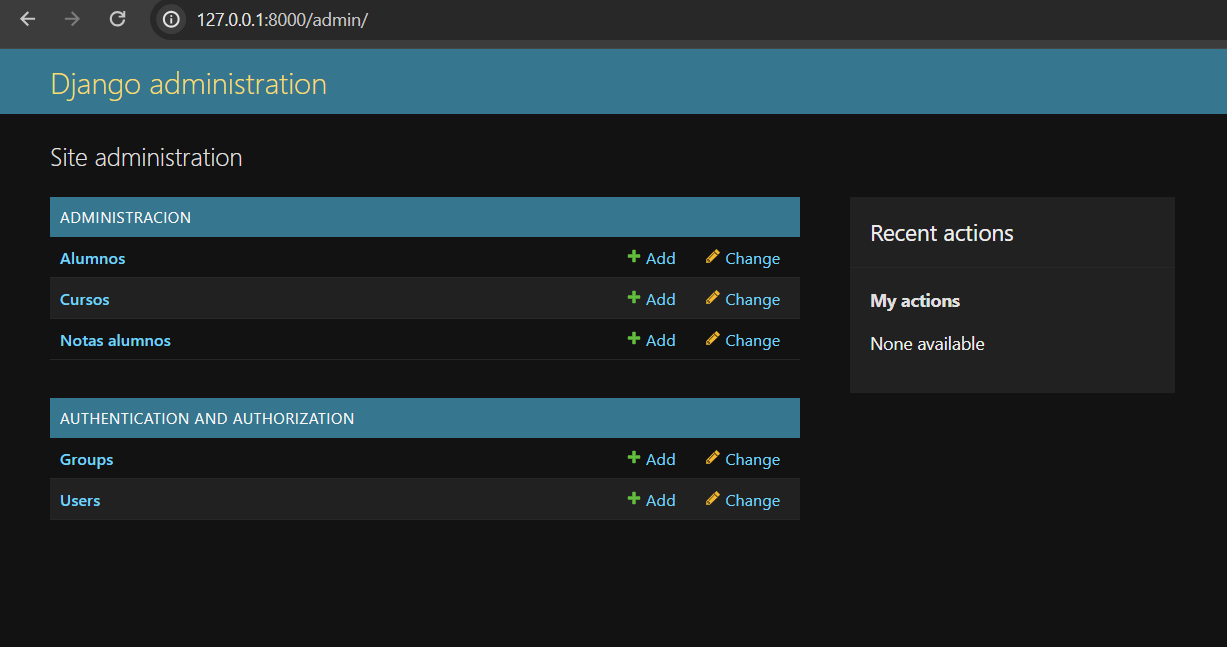
\includegraphics[width=0.8\textwidth,keepaspectratio]{Ejecucion de servidor en desarrollo.png}
        
        \item ARCHIVOS MODIFICADOS (PROYECTO)
        
        \begin{lstlisting}[language=Python, caption=settings.py]
"""
Django settings for ejercicioPropuesto project.

Generated by 'django-admin startproject' using Django 5.0.6.

For more information on this file, see
https://docs.djangoproject.com/en/5.0/topics/settings/

For the full list of settings and their values, see
https://docs.djangoproject.com/en/5.0/ref/settings/
"""

from pathlib import Path
import os

# Build paths inside the project like this: BASE_DIR / 'subdir'.
BASE_DIR = Path(__file__).resolve().parent.parent


# Quick-start development settings - unsuitable for production
# See https://docs.djangoproject.com/en/5.0/howto/deployment/checklist/

# SECURITY WARNING: keep the secret key used in production secret!
SECRET_KEY = 'django-insecure-@d%raj871b-2=5vz#hep+1pfvd+e27)0!)wj!u6$!@ic10e5@u'

# SECURITY WARNING: don't run with debug turned on in production!
DEBUG = True

ALLOWED_HOSTS = []


# Application definition

INSTALLED_APPS = [
    'django.contrib.admin',
    'django.contrib.auth',
    'django.contrib.contenttypes',
    'django.contrib.sessions',
    'django.contrib.messages',
    'django.contrib.staticfiles',

    #APPS PROPIAS
    'administracion'
]

MIDDLEWARE = [
    'django.middleware.security.SecurityMiddleware',
    'django.contrib.sessions.middleware.SessionMiddleware',
    'django.middleware.common.CommonMiddleware',
    'django.middleware.csrf.CsrfViewMiddleware',
    'django.contrib.auth.middleware.AuthenticationMiddleware',
    'django.contrib.messages.middleware.MessageMiddleware',
    'django.middleware.clickjacking.XFrameOptionsMiddleware',
]

ROOT_URLCONF = 'ejercicioPropuesto.urls'

TEMPLATES = [
    {
        'BACKEND': 'django.template.backends.django.DjangoTemplates',
        'DIRS': [os.path.join(BASE_DIR, 'templates')],
        'APP_DIRS': True,
        'OPTIONS': {
            'context_processors': [
                'django.template.context_processors.debug',
                'django.template.context_processors.request',
                'django.contrib.auth.context_processors.auth',
                'django.contrib.messages.context_processors.messages',
            ],
        },
    },
]

WSGI_APPLICATION = 'ejercicioPropuesto.wsgi.application'


# Database
# https://docs.djangoproject.com/en/5.0/ref/settings/#databases

DATABASES = {
    'default': {
        'ENGINE': 'django.db.backends.sqlite3',
        'NAME': BASE_DIR / 'db.sqlite3',
    }
}


# Password validation
# https://docs.djangoproject.com/en/5.0/ref/settings/#auth-password-validators

AUTH_PASSWORD_VALIDATORS = [
    {
        'NAME': 'django.contrib.auth.password_validation.UserAttributeSimilarityValidator',
    },
    {
        'NAME': 'django.contrib.auth.password_validation.MinimumLengthValidator',
    },
    {
        'NAME': 'django.contrib.auth.password_validation.CommonPasswordValidator',
    },
    {
        'NAME': 'django.contrib.auth.password_validation.NumericPasswordValidator',
    },
]


# Internationalization
# https://docs.djangoproject.com/en/5.0/topics/i18n/

LANGUAGE_CODE = 'en-us'

TIME_ZONE = 'UTC'

USE_I18N = True

USE_TZ = True


# Static files (CSS, JavaScript, Images)
# https://docs.djangoproject.com/en/5.0/howto/static-files/

STATIC_URL = 'static/'

# Default primary key field type
# https://docs.djangoproject.com/en/5.0/ref/settings/#default-auto-field

DEFAULT_AUTO_FIELD = 'django.db.models.BigAutoField'

        \end{lstlisting} 

        \begin{lstlisting}[language=Python, caption=urls.py]
from django.contrib import admin
from django.urls import path, include

urlpatterns = [
    path('admin/', admin.site.urls),
    path('administracion/', include('administracion.urls')),
]

        \end{lstlisting} 

    \clearpage

	\section{\textcolor{red}{Rúbricas}}
	
	\subsection{\textcolor{red}{Entregable Informe}}
	\begin{table}[H]
		\caption{Tipo de Informe}
		\setlength{\tabcolsep}{0.5em} % for the horizontal padding
		{\renewcommand{\arraystretch}{1.5}% for the vertical padding
		\begin{tabular}{|p{3cm}|p{12cm}|}
			\hline
			\multicolumn{2}{|c|}{\textbf{\textcolor{red}{Informe}}}  \\
			\hline 
			\textbf{\textcolor{red}{Latex}} & \textcolor{blue}{El informe está en formato PDF desde Latex,  con un formato limpio (buena presentación) y facil de leer.}   \\ 
			\hline 
			
			
		\end{tabular}
	}
	\end{table}
	

	
	\subsection{\textcolor{red}{Rúbrica para el contenido del Informe y demostración}}
	\begin{itemize}			
		\item El alumno debe marcar o dejar en blanco en celdas de la columna \textbf{Checklist} si cumplio con el ítem correspondiente.
		\item Si un alumno supera la fecha de entrega,  su calificación será sobre la nota mínima aprobada, siempre y cuando cumpla con todos lo items.
		\item El alumno debe autocalificarse en la columna \textbf{Estudiante} de acuerdo a la siguiente tabla:
	
		\begin{table}[ht]
			\caption{Niveles de desempeño}
			\begin{center}
			\begin{tabular}{ccccc}
    			\hline
    			 & \multicolumn{4}{c}{Nivel}\\
    			\cline{1-5}
    			\textbf{Puntos} & Insatisfactorio 25\%& En Proceso 50\% & Satisfactorio 75\% & Sobresaliente 100\%\\
    			\textbf{2.0}&0.5&1.0&1.5&2.0\\
    			\textbf{4.0}&1.0&2.0&3.0&4.0\\
    		\hline
			\end{tabular}
		\end{center}
	\end{table}	
	
	\end{itemize}
	
	\begin{table}[H]
		\caption{Rúbrica para contenido del Informe y demostración}
		\setlength{\tabcolsep}{0.5em} % for the horizontal padding
		{\renewcommand{\arraystretch}{1.5}% for the vertical padding
		%\begin{center}
		\begin{tabular}{|p{2.7cm}|p{7cm}|x{1.3cm}|p{1.2cm}|p{1.5cm}|p{1.1cm}|}
			\hline
    		\multicolumn{2}{|c|}{Contenido y demostración} & Puntos & Checklist & Estudiante & Profesor\\
			\hline
			\textbf{1. GitHub} & Hay enlace URL activo del directorio para el  laboratorio hacia su repositorio GitHub con código fuente terminado y fácil de revisar. &2 &X &2 & \\ 
			\hline
			\textbf{2. Commits} &  Hay capturas de pantalla de los commits más importantes con sus explicaciones detalladas. (El profesor puede preguntar para refrendar calificación). &4 &X &2 &  \\ 
			\hline 
			\textbf{3. Código fuente} &  Hay porciones de código fuente importantes con numeración y explicaciones detalladas de sus funciones. &2 &X &2 & \\ 
			\hline 
			\textbf{4. Ejecución} & Se incluyen ejecuciones/pruebas del código fuente  explicadas gradualmente. &2 &X &1 & \\ 
			\hline			
			\textbf{5. Pregunta} & Se responde con completitud a la pregunta formulada en la tarea.  (El profesor puede preguntar para refrendar calificación).  &2 &X &2 & \\ 
			\hline	
			\textbf{6. Fechas} & Las fechas de modificación del código fuente estan dentro de los plazos de fecha de entrega establecidos. &2 &X &2 & \\ 
			\hline 
			\textbf{7. Ortografía} & El documento no muestra errores ortográficos. &2 &X &2 & \\ 
			\hline 
			\textbf{8. Madurez} & El Informe muestra de manera general una evolución de la madurez del código fuente,  explicaciones puntuales pero precisas y un acabado impecable.   (El profesor puede preguntar para refrendar calificación).  &4 &X &4 & \\ 
			\hline
			\multicolumn{2}{|c|}{\textbf{Total}} &20 & &17 & \\ 
			\hline
		\end{tabular}
		%\end{center}
		%\label{tab:multicol}
		}
	\end{table}
	
\clearpage
	
	
%\clearpage
%\bibliographystyle{apalike}
%\bibliographystyle{IEEEtranN}
%\bibliography{bibliography}
			
\end{document}